% To je predloga za poročila o domačih nalogah pri predmetih, katerih
% nosilec je Blaž Zupan. Seveda lahko tudi dodaš kakšen nov, zanimiv
% in uporaben element, ki ga v tej predlogi (še) ni. Več o LaTeX-u izveš na
% spletu, na primer na http://tobi.oetiker.ch/lshort/lshort.pdf.
%
% To predlogo lahko spremeniš v PDF dokument s pomočjo programa
% pdflatex, ki je del standardne instalacije LaTeX programov.

\documentclass[a4paper,11pt]{article}
\usepackage{a4wide}
\usepackage{fullpage}
\usepackage[utf8x]{inputenc}
\usepackage[slovene]{babel}
\selectlanguage{slovene}
\usepackage[toc,page]{appendix}
\usepackage[pdftex]{graphicx} % za slike
\usepackage{setspace}
\usepackage{color}
\definecolor{light-gray}{gray}{0.95}
\usepackage{listings} % za vključevanje kode
\usepackage{hyperref}
\usepackage{float}
\renewcommand{\baselinestretch}{1.2} % za boljšo berljivost večji razmak
\renewcommand{\appendixpagename}{Priloge}

\lstset{ % nastavitve za izpis kode, sem lahko tudi kaj dodaš/spremeniš
language=Python,
basicstyle=\footnotesize,
basicstyle=\ttfamily\footnotesize\setstretch{1},
backgroundcolor=\color{light-gray},
}

\title{Inteligentni sistemi, 1. seminarska naloga}
\author{Matic Bernik in Robert Tovornik}
\date{\today}

\begin{document}

\maketitle

\section{Uvod}

Namen seminarske naloge je, da na podlagi podanih podaktov tekem NBA, 
zgradimo napovedni model, ga preverimo, ter z njim napovemo zmagovalca 
nove, prihodnje tekme, ter končno razliiko točk v koših med ekipama.

\section{Podatki}

V okviru seminarske naloge, so nam bili podani podatki tekem v NBA za pretekli 
 sezoni 2008/09 ter 2009/10. Ti se nahajajo v dveh datotekah: \\

\textendash  nba0809.txt 

\textendash  nba0910.txt

Skupaj obsegajo 2459 primerov, ter so opisani z 31 začetnimi atributi.
Med podatki ni mankajoči vrednosti (N/A).

\section{Pregled podatkov}

Ob zacetku, sva pregledala razporeditev podanih podatkov, s pomocjo orodja 
ORANGE (razvit na FRI), ter ugotovila, da so podatki razporejeni normalno, kar
 je zaželjeno ( razen podatkov o home in away team ).

\begin{figure}[H]
\begin{center}
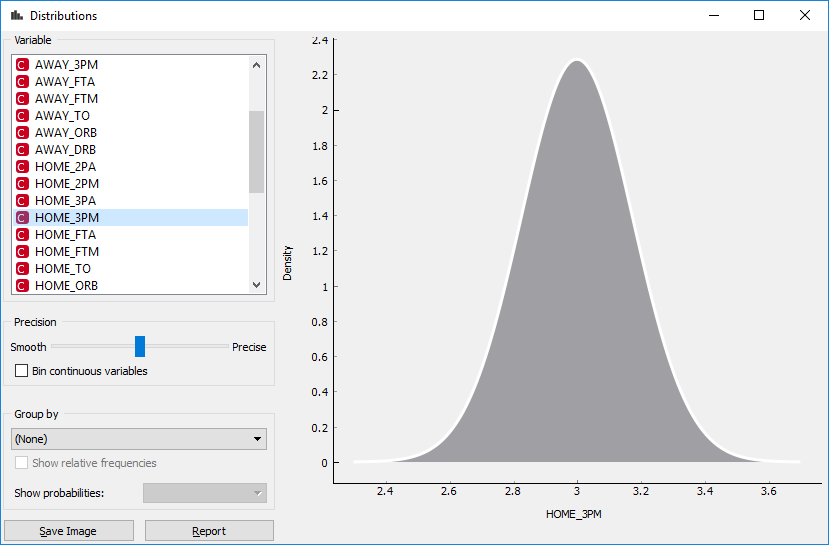
\includegraphics[scale=0.3]{OC_data_dist.png}
\caption{Prikaz razporeditve posamezni podatkov v orodju Orange (distributions).}
\label{slika1}
\end{center}
\end{figure} 

\section{Iskanje napovednih atributov}

Da bi lažje določila pomembnost atributov, ki določajo rezultat tekme, sva 
uporabila orodje Orange, za izračun teže informacije, oziroma ocene koliko 
določen atribut doprinese h končni napovedi. Le-te sva izračunala z ocenami atributov: 
 "Information gain", "Gain Ratio", "Gini" ter "ReliefF".

\begin{figure}[H]
\begin{center}
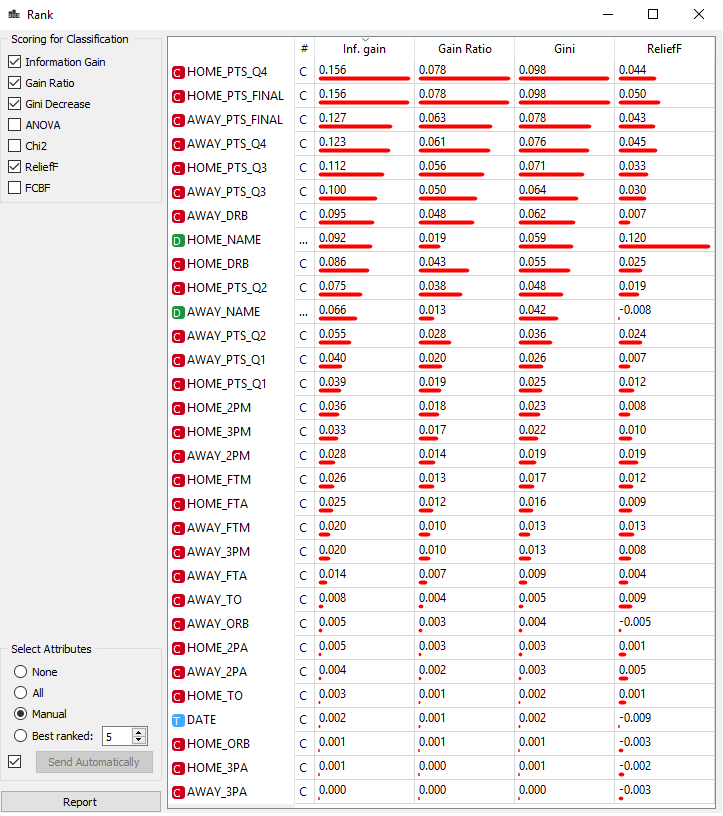
\includegraphics[scale=0.3]{OC_ranking_by_inf_gain.png}
\caption{Ocena teže oziroma informacijskega doprinosa atributov k napovedi.}
\label{slika2}
\end{center}
\end{figure} 

Presenetilo naju je, da poleg uspešnosti zadevanja koša, močno vplivajo tudi nekateri 
drugi atributi, med katerimi močno izstopa attribut "Defensive Rebounds". Po dodatnem testu, 
s funkcionalnostjo scatter plot, se je izkazalo, da močno nakazuje na končno število zadetih košev.

\begin{figure}[H]
\begin{center}
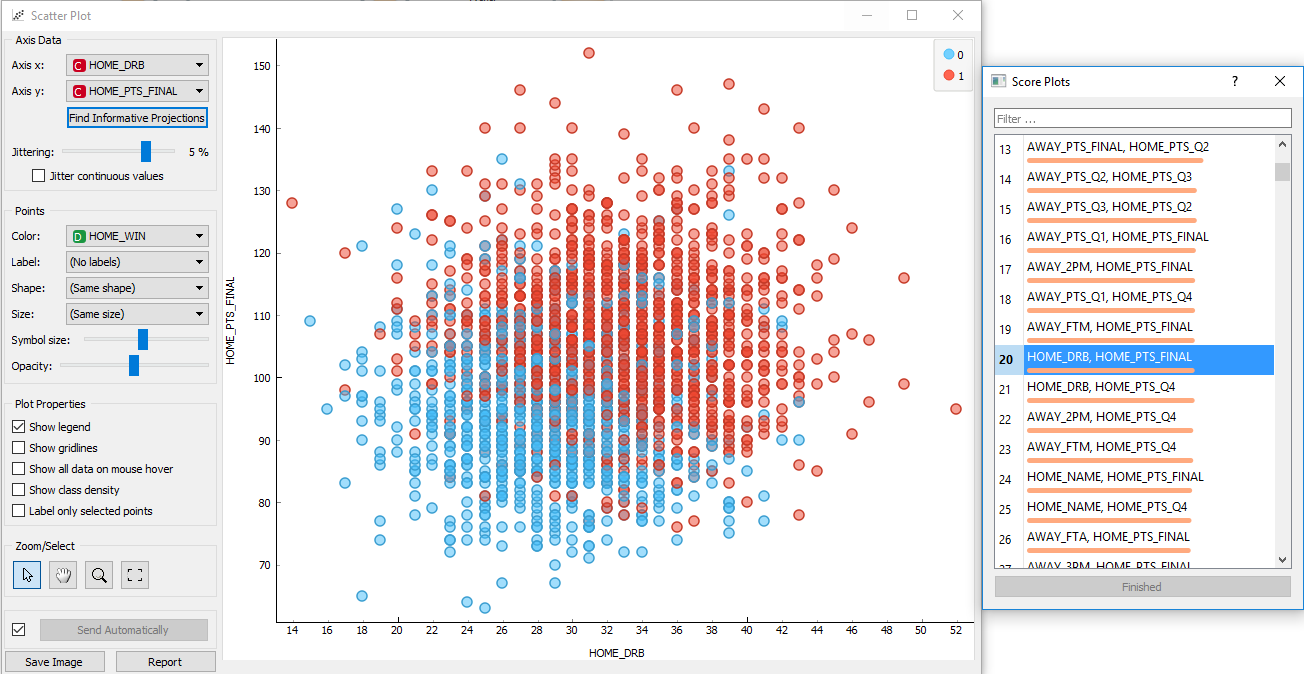
\includegraphics[scale=0.3]{OC_DRB_PTS-FINAL.png}
\caption{Scatter plot - relacija med "Defensive rebounds" in "Final points scored".}
\label{slika2.1}
\end{center}
\end{figure} 


\section{Ustvarjanje novih atributov}

Ko sva ocenila informacijske lastnosti atributov, sva se lotila iskanja možnosti združevanja 
in prepoznavanja sorodnosti atributov. Za to sva uporabila funkcionalnost orodja Orange,
HeatMap, ter hkrati clustering in opazila anomalijo, ki jo povzroča datum, ki tekme unikatno
 določa. Zato sva le-tega odstranila iz učnih podatkov, ter ponovno zagnala prepoznavanje.\\



\begin{figure}[H]
    \centering
    \begin{minipage}{0.5\textwidth}
        \centering
        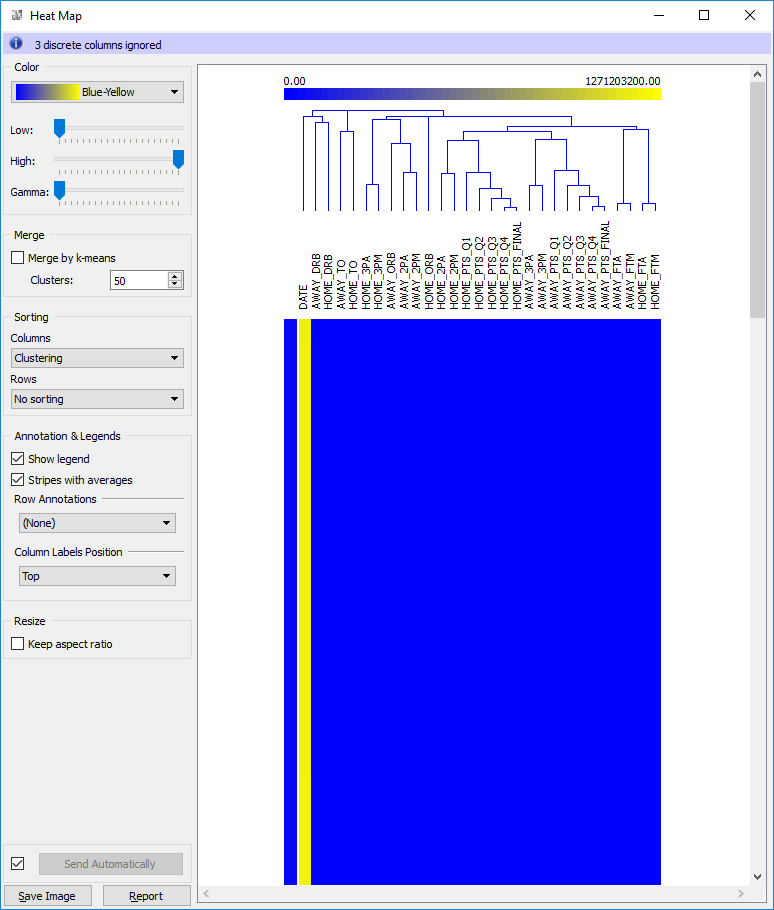
\includegraphics[width=0.9\textwidth]{OC_attrib-cluster.png}
        \caption{Heatmap z datumom}
        \label{slika3}
    \end{minipage}\hfill
    \begin{minipage}{0.5\textwidth}
        \centering
        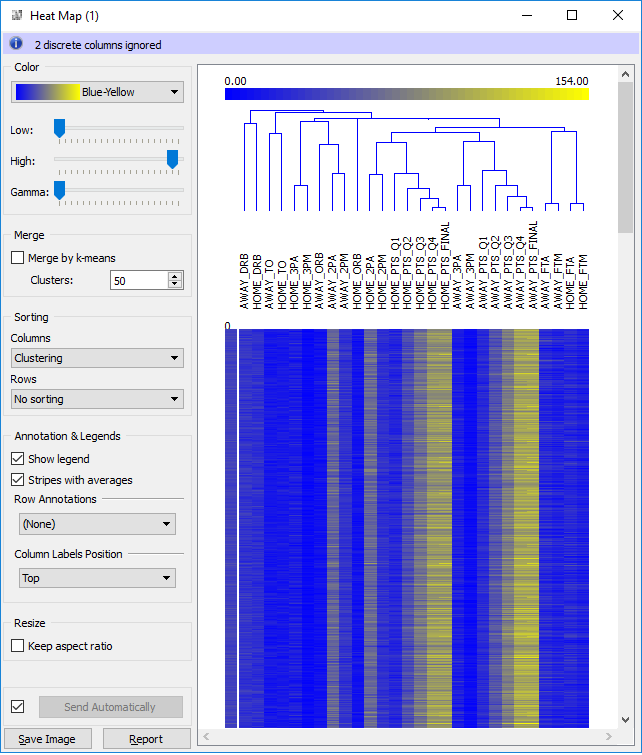
\includegraphics[width=0.9\textwidth]{OC_attrib-cluster-no_date.png}
        \caption{Heatmap, datum odstranjen}
        \label{slika4}
    \end{minipage}
\end{figure}



\section{Metode}

Tu opišeš, na kakšen način si rešil nalogo (tehnike in metode, ki si
jih uporabil). Lahko vključiš tudi zanimiv del programske kode, ki
si jo morda pri tem razvil ali pa v poročilo dodatno vključiš sliko,
kot je na primer slika~\ref{slika1}. Vse slike in tabele, ki jih
vključiš v poročilo, morajo biti navedene v besedilu oziroma se moraš
na njih sklicati.

\begin{figure}[htbp]
\begin{center}
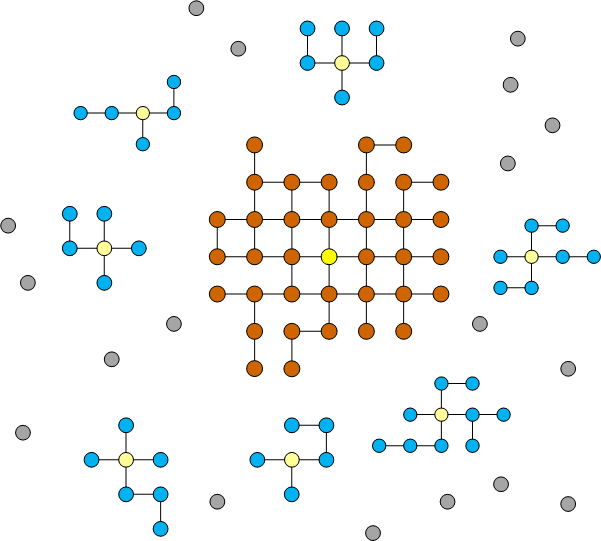
\includegraphics[scale=0.3]{slika-primer.png}
\caption{Vsako sliko opremi s podnapisom, ki pove, kaj slika prikazuje.}
\label{slika1}
\end{center}
\end{figure}

V to poglavje lahko tudi vključiš kakšen metodološko zanimiv del
kode. Primer vključitve kode oziroma implementirane funkcije v
programskem jeziku Python je:

\begin{lstlisting}
def fib(n):
    if n == 0:
        return 0
    elif n == 1:
        return 1
    else:
        return fib(n-1) + fib(n-2)
\end{lstlisting}

Izris te kode je lahko sicer tudi lepši, poskušaš lahko najti še
primernejši način vključevanja kode v Pythonu oziroma v tvojem izbranem
programskem jeziku v okolje \LaTeX{}.

\section{Rezultati}

V tem poglavju podaš rezultate s kratkim (enoodstavčnim)
komentarjem. Rezultate lahko prikažeš tudi v tabeli (primer je
tabela~\ref{tab1}).

Odstavke pri pisanju poročila v LaTeX-u ločiš tako, da pred novim
odstavkom pustiš prazno vrstico. Tudi, če pišeš poročilo v kakšnem
drugem urejevalniku, morajo odstavki biti vidno ločeni. To narediš z
zamikanjem ali pa z dodatnim presledkom.

\begin{table}[htbp]
\caption{Atributi in njihove zaloge vrednosti.}
\label{tab1}
\begin{center}
\begin{tabular}{llp{3cm}}
\hline
ime spremenljivke & definicijsko območje & opis \\
\hline
cena & [0, 500] & cena izdelka v EUR\\
teža & [1, 1000] & teža izdelka v dag \\
kakovost & [slaba|srednja|dobra] & kakovost izdelka \\
\hline
\end{tabular}
\end{center}
\end{table}

Podajanje rezultati naj bo primerno strukturirano. Če ima naloga več
podnalog, uporabi podpoglavja. Če bi želel poročati o rezultatih
izčrpno in pri tem uporabiti vrsto tabel ali grafov, razmisli o
varianti, kjer v tem poglavju prikažeš in komentiraš samo glavne
rezultate, kakšne manj zanimive detajle pa vključite v prilogo (glej
prilogi~\ref{app-res} in~\ref{app-code}).

\section{Izjava o izdelavi domače naloge}
Domačo nalogo in pripadajoče programe sem izdelal sam.

\appendix
\appendixpage
\section{\label{app-res}Podrobni rezultati poskusov}

Če je rezultatov v smislu tabel ali pa grafov v nalogi mnogo,
predstavi v osnovnem besedilu samo glavne, podroben prikaz
rezultatov pa lahko predstaviš v prilogi. V glavnem besedilu ne
pozabi navesti, da so podrobni rezultati podani v prilogi.

\section{\label{app-code}Programska koda}

Za domače naloge bo tipično potrebno kaj sprogramirati. Če ne bo od
vas zahtevano, da kodo oddate posebej, to vključite v prilogo. Čisto
za okus sem tu postavil nekaj kode, ki uporablja Orange
(\url{http://www.biolab.si/orange}) in razvrščanje v skupine.


\begin{lstlisting}
import random
import Orange

data_names = ["iris", "housing", "vehicle"]
data_sets = [Orange.data.Table(name) for name in data_names]

print "%10s %3s %3s %3s" % ("", "Rnd", "Div", "HC")
for data, name in zip(data_sets, data_names):
    random.seed(42)
    km_random = Orange.clustering.kmeans.Clustering(data, centroids = 3)
    km_diversity = Orange.clustering.kmeans.Clustering(data, centroids = 3,
        initialization=Orange.clustering.kmeans.init_diversity)
    km_hc = Orange.clustering.kmeans.Clustering(data, centroids = 3,
        initialization=Orange.clustering.kmeans.init_hclustering(n=100))
    print "%10s %3d %3d %3d" % (name, km_random.iteration, \
    km_diversity.iteration, km_hc.iteration)
\end{lstlisting}

\end{document}
